\section*{Экспоненциальное семейство распределений}
Всегда ранее мы предполагали наша модель $f(\cdot, \alpha)$ предсказывает мир с какой-то ошибкой, т.е.
$$
y_i = f(x_i, \alpha) + \varepsilon_i,
$$
где $\varepsilon_i \sim \mathcal{N}(0, \sigma_i^2)$. Тоесть ошибка распределена нормально. Однако в общем случае это может быть не так и ошибка может быть приходить из какого-то другого распределения, что пораждает другое распределение и у самих $y_i$. Долее будем считать, что распределение ошибок приходит из экспоненциального семейства.

\noindent\textbf{Определение.} Распределение $\mathsf{P}$ принадлежит \textit{экспоненциальному семейству} ($\mathsf{Exp}(\theta_i, \phi_i)$) с параметрами $\theta_i, \phi_i$ и параметрами-функциями $c(\theta), h(y, \phi)$, если его пролтность представляется в следующем виде:
$$
p(y_i) = \exp\left(
  \frac{y_i\theta_i - c(\theta_i)}{\phi_i} + h(y_i, \phi_i)
\right)
$$.
Предполагается, что $c(\theta)$ - непрерывно дважды дифференцируема, $c'(\theta)$ - монотонна, а $h(y, \phi)$ - непрерывна по $y$.

Пусть $y_i \sim \mathsf{Exp}(\theta_i, \phi_i)$, тогда
\begin{align*}
  \mu_i := \mathsf{E}y_i &= c'(\theta_i)\\
  \mathsf{D}y_i &= \frac{c''(\theta_i)}{\phi_i}
\end{align*}

\noindent\textbf{Определение.} \textit{Функцией связи} называется функция обратная $c'(\theta_i)$.
$$
g(\mu_i) = (c')^{-1}(\mu_i) \text{ - функция связи.}
$$

Несмотря на то, что распределений из экспоненциального семейства мало - на практике выходит так, что почти всякое распределение - экспоненциально.

\section*{Принцип максимального правдоподобия для GLM}
В случае, если нам известно, что величины $y_i$ не из нормального распределения, но из экспоненциального - пользоваться методом наименьших квадратов нельзя. Нужно честно выписывать принцип максимального правдоподобия.
Пусть $y_i \sim \mathsf{Exp}(\theta_i, \phi_i)$. Выпишем функцию правдоподобия.
$$
L(\alpha) = \ln \prod_{i=1}^l p(y_i \mid \theta_i, \phi_i) = \sum_{i=1}^l \frac{y_i \theta_i - c(\theta_i))}{\phi_i} + h(y_i, \phi_i) \to \max_\alpha.
$$
Если дополнительно известно, что выборка гомоскедастична (тоесть все $\phi_i$ равны), то слагаемое $h(y_i, \phi_i)$ - можно убрать, ак как $h$ не зависет ни от объектов, ни от параметров модели.

Из постановки GLM мы знаем, что $\theta_i = x_i^\top\alpha$.

Будем находить максимум правдоподобия методом Ньютона-Рафсона
$$
\alpha^{t+1} = \alpha^t + h_t \left(L''(\alpha^t)\right)^{-1}L'(\alpha^t).
$$
Явно выпишем эти матрицы:
$$
\frac{\partial L(\alpha)}{\partial \alpha_j} = \sum_{i=1}^l \frac{y_i - c'(x_i^\top\alpha)}{\phi_i}f_j(x_i)
$$
$$
\frac{\partial^2 L(\alpha)}{\partial \alpha_j\partial \alpha_k} = \sum_{i=1}^l \frac{c''(x_i^\top\alpha)}{\phi_i}f_j(x_i)f_k(x_i)
$$
Можно заметить, что $L''(\alpha)$ можно представить, как произведение трех матриц - одной диагональной, и двух матриц "объект-признак".
$$
L''(\alpha) = F^\top D_t F,
$$
где $F$ - матрица "объект-признак", а $D_t$ - диагональна, $[D_t]_{i,i} = \frac{c''(x_i^\top\alpha^t)}{\phi_i}$.
Матрицу $D_t$ можно разделить на две и каждую из частей присоеденить к $F$:
\begin{align*}
  D_t &= W_t W_t & W_t &= \sqrt{D_t}\\
  L''(\alpha) &= F^\top D_t F = \widetilde{F}^\top\widetilde{F} & \widetilde{F} &= W_t F.
\end{align*}.
Теперь преобразуем вектор $L'(\alpha)$. Можно его представить как произведение $\widetilde{F}$ на другой вектор $\widetilde{y}^t$.
\begin{align*}
  L'(\alpha) &= \widetilde{F}\widetilde{y}^t & \widetilde{y}^t_i &= \frac{y_i - c'(x_i^\top\alpha^t)}{\sqrt{\phi_i c''(x_i^\top\alpha^t)}}
\end{align*}
Этот вектор $\widetilde{y}^t$ можно воспринимать как отнормированный вектор ответов. Если вспонить, что $\mathsf{E}(y_i) = c'(\theta_i)$, $\mathsf{D}(y_i) = c''(\theta_i)$, а $\theta_i = x^\top \alpha$, то получается, что $\widetilde{y}^t$ - как раз стандатная нормировка $y$ в предположении, что он взят из распределения $\mathsf{Exp}(x^\top \alpha^t, \phi_i)$.

Тогда итерацию в методе Ньютона-Рафсона можно записать так
$$
\alpha^{t+1} = \alpha^t + h_t \left(L''(\alpha^t)\right)^{-1}L'(\alpha^t) =
\alpha^t + h_t \left(\widetilde{F}^\top\widetilde{F}\right)^{-1}\widetilde{F}\widetilde{y}^t
$$
Но тогда мы получили новую задачу регрессии
$$
Q(\alpha) = \|\widetilde{F} \alpha - \widetilde{y}^t\|^2 \to \min_{\alpha}.
$$
$\alpha^{t+1}$ является решением задачи выше. Таким образом, иттеративно подбирая $\alpha^t$ метод сойдется к некоторому значению $\alpha$, которое и будет являться решением регрессии методом максимального правдоподобия.

\section*{Логистическая регрессия как частный случай GLM}
Рассмотрим задачу регрессии. Сделаем всего 2 предположения:
\begin{enumerate}
  \item $y_i$ - бернулевские случайные величины. Тоесть у $y_i$ есть вероятность быть в том или ином классе.
  \item Модель линейна и $\mu_i = \mathsf{E}y_i$ монотонно зависет от $\theta_i = x_i^\top\alpha$.
\end{enumerate}
Лишь из этих двух предположений мы сразу получаем функцию связи
$$
\theta_i = \gamma(\mu_i) = \ln\frac{\mu_i}{1-\mu_i}
$$
$$
\mu_i = c'(\theta_i) = \frac{1}{1+\exp(\theta_i)} = \sigma(-\theta_i) \text{ - сигмойда}.
$$
Записывая же метод максимального правдоподобия, получаем минимизацию критерия negative-log-loss.
$$
-L(\alpha) = -\sum_{i=1}^l \ln p(y_i \mid x_i) = \sum_{i=1}^l -y_i \ln \mu_i + (y_i - 1) \ln (1 - \mu_i) \to \min_\alpha
$$
Распишем случаи для $y_i$
$$
\ln p(y_i \mid x_i) = 
\begin{cases}
  \ln\mu_i = \ln(\sigma(\theta_i)) = \ln(\sigma(x_i^\top\alpha)) & y_i = 1\\
  \ln(1 - \mu_i) = \ln(\sigma(-\theta_i)) = \ln(\sigma(-x_i^\top\alpha)) & y_i = 0
\end{cases} = \ln(\sigma(\widetilde{y}_ix_i^\top\alpha)),
$$
где $\widetilde{y}_i = 2y_i - 1$. Тогда принцип максимального правдоподобия можно перепиcать как
$$
-L(\alpha) = \sum_{i=1}^l -\ln(\sigma(\widetilde{y}_ix_i^\top\alpha)) = 
\sum_{i=1}^l \ln(1 + \exp(-\widetilde{y}_ix_i^\top\alpha)).
$$

\subsection*{Задача 1}

Доказать, что если $y_i \sim \mathsf{Exp}(\theta_i, \phi_i)$, существует матожидание и дисперсия $y_i$ и выполены условия на $c(\theta)$, $h(y, \phi)$, то
\begin{align*}
  \mathsf{E}y_i &= c'(\theta_i)\\
  \mathsf{D}y_i &= \frac{c''(\theta_i)}{\phi_i}
\end{align*}

\begin{proof}
  Рассмотрим функцию
  $$
  f(y_i, \theta) = \exp\left(
  \frac{y_i\theta - c(\theta)}{\phi_i} + h(y_i, \phi_i)\right).
  $$
  Тогда $p(y_i) = f(y_i, \theta_i) \geq 0$. Из условий на $c(\theta)$ и $h(y_i, \phi_i)$ получаем, что $f(y_i, \theta)$ непрерывна вместе со своей частной производной $\frac{\partial f}{\partial \theta}(y_i, \theta)$. Хотим продифференцировать интеграл от $f$, для этого рассмотрим прямоугольник $[-n, n]\times[\alpha, \beta] \ni (y_i, \theta_i)$. Тогда верно, что
  $$
  \frac{\partial}{\partial\theta} \int_{-n}^n f(y_i, \theta)\,dy_i = \int_{-n}^n\frac{\partial f}{\partial\theta}(y_i,\theta)\,dy_i.
  $$
  
  Разберемся сначала с правой частью.
  \begin{multline*}
    \int_{-n}^n\frac{\partial f}{\partial\theta}(y_i,\theta)\,dy_i =
    \int_{-n}^n\frac{y_i - c'(\theta)}{\phi_i} f(y_i, \theta)\,dy_i =\\=
    \frac{1}{\phi}
    \underbrace{
      \int_{-n}^n y_if(y_i, \theta)\,dy_i
    }_{\to\mathsf{E}_\theta y_i \text{ при } n\to\infty} +
    \frac{c'(\theta)}{\phi}
    \underbrace{
      \int_{-n}^n f(y_i, \theta)\,dy_i
    }_{\to 1 \text{ при } n\to\infty}\to
    \frac{\mathsf{E}_\theta y_i - c'(\theta)}{\phi_i} \text{ при } n\to\infty,
  \end{multline*}
  Причем не трудно видеть, что сходимость равномерная.
  
  Теперь разберемся с левой частью. Мы уже знаем, что
  $$
  \int_{-n}^n\frac{\partial f}{\partial\theta}(y_i,\theta)\,dy_i \rightrightarrows \frac{\mathsf{E}_\theta y_i - c'(\theta)}{\phi_i} \text{ при } n\to\infty,
  $$
  Но тогда можно делать предельный переход под знаком производной!
  $$
  \frac{\partial}{\partial\theta} \int_{-n}^n f(y_i, \theta)\,dy_i \to \frac{\partial}{\partial\theta} \int_{-\infty}^\infty f(y_i, \theta)\,dy_i = \frac{\partial}{\partial\theta} 1 = 0 \text{ при } n\to\infty.
  $$
  Приравнивая левую и правую части в точке $\theta_i$, получаем
  $$
  0 = \frac{\mathsf{E}y_i - c'(\theta_i)}{\phi_i},
  $$
  $$
  \mathsf{E}y_i = c'(\theta_i).
  $$
  Для того, чтобы разобраться с дисперсией нужно проделать все тоже самое, только с $\frac{\partial f}{\partial\theta}(y_i, \theta)$, вместо $f(y_i, \theta)$. Имеем
  $$
  \frac{\partial^2}{\partial\theta^2} \int_{-n}^n f(y_i, \theta)\,dy_i =
  \frac{\partial}{\partial\theta} \int_{-n}^n\frac{\partial f}{\partial\theta}(y_i,\theta)\,dy_i = \int_{-n}^n\frac{\partial^2 f}{\partial\theta^2}(y_i,\theta)\,dy_i.
  $$
  Вновь начнем с правой части и аналогично получим
  \begin{multline*}
    \int_{-n}^n\frac{\partial^2 f}{\partial\theta^2}(y_i,\theta)\,dy_i =
    \int_{-n}^n \frac{y_i^2 - 2y_ic'(\theta) + c'(\theta)^2 - c''(\theta)\phi_i}{\phi_i^2} f(y_i,\theta)\,dy_i \rightrightarrows\\
    \rightrightarrows
    \frac{1}{\phi_i^2}\mathsf{E}_\theta y_i^2 -
    \frac{2c'(\theta)}{\phi_i^2}\mathsf{E}_\theta y_i +
    \frac{c'(\theta)^2 - c''(\theta)\phi_i}{\phi_i^2} \text{ при } n\to\infty.
  \end{multline*}
  В левой части аналогично предел равен нулю. Приравнивая все в точке $\theta_i$ получаем
  $$
  0 = \frac{1}{\phi_i^2}\mathsf{E} y_i^2 -
  \frac{2c'(\theta_i)}{\phi_i^2}\mathsf{E} y_i +
  \frac{c'(\theta_i)^2 - c''(\theta_i)\phi_i}{\phi_i^2}
  $$
  Не забудем, что $c'(\theta_i) = \mathsf{E} y_i$.
  $$
  0 = \mathsf{E} y_i^2 - 2\left(\mathsf{E} y_i\right)^2 + \left(\mathsf{E} y_i\right)^2 - c''(\theta_i)\phi_i
  $$
  $$
  c''(\theta_i)\phi_i = \mathsf{E} y_i^2 - \left(\mathsf{E} y_i\right)^2 = \mathsf{D}y_i
  $$
\end{proof}

\subsection*{Задача 2}

Компания aperture science занимается разработкой и тестированием портальных устройств. Перед тестом находится подопытный человек, специальная комманда исследователей точно измеряют его характеристики такие как: рост, iq и объективная оценка привлекательности (от -7 до 100). Испытуемому выдают портальную пушку и запускают в комнату тестирования. Про нее тоже есть информация: общий объем комнаты, сложность испытания, количество камер и количество турелей. Отдельно обученная группа математиков подсчитывала количетсво открытых порталов во время первых 10 миинут тестирования. Этой величиной называют pq испытуемого (или portal quotient). Поскольку портальная пушка - крайне энергозатратное устройство - компания нанимает отдельную группу аналитиков для того, чтобы по уже имеющимся данным предсказывать pq испытуемого и не допускать до тестирования тех, чей pq окажется слишком большим.

Необходимо получить регрессионную модель с помощью принципа максимального правдоподобия и построить GLM, которые по данным $x_i$ будут предсказывать $pq_i$. Считать, что $pq_i \sim \text{Pois}(\lambda_i)$.

\noindent\textit{Решение.}
Пуассоновское распределение принадлежит экспоненциальному семейству, действительно
$$
p(pq_i \mid \lambda_i) = \frac{e^{-\lambda_i}\lambda_i^{pq_i}}{pq_i!} = \exp\left(
pq_i\ln(\lambda_i) - \lambda_i - \ln(pq_i!)
\right),
$$
Причем параметры равны
\begin{align*}
  \theta_i &= \ln(\lambda_i),\\
  c(\theta_i) &= \lambda_i = e^\theta_i,\\
  \phi_i &= 1.
\end{align*}
Функция связи при этом равна
\begin{align*}
  \mu_i &= c'(\theta_i) = e^\theta_i &
  \theta_i = g(\mu_i) = \ln(\mu_i)
\end{align*}

Воспользуемся методом максимального правдоподобия:
$$
-L(\alpha) = -\sum_{i=1}^l \ln p(pq_i \mid \mu_i) = -\sum_{i=1}^l pq_i \theta_i - \mu_i =
\sum_{i=1}^l \exp\left(x_i^\top \alpha\right) - pq_i \cdot x_i^\top \alpha \to \min_\alpha
$$
Тогда для решения можно просто обучить линейную регрессию с функцией потерь, описаной выше.

Посмотрим также как бы выглядела MSE-регрессия, полученая в методе Ньютона-Рафсона.
$$
[W_t]_{i,i} = \sqrt{\frac{c''(x_i^\top\alpha^t)}{\phi_i}} = \exp\left(\frac{x_i^\top\alpha^t}{2}\right)
$$
$$
[\widetilde{F}]_{i,j} = f_i(x_j)\exp\left(\frac{x_j^\top\alpha^t}{2}\right)
$$
$$
\widetilde{y}^t_i = \frac{y_i - c'(x_i^\top\alpha^t)}{\sqrt{\phi_i c''(x_i^\top\alpha^t)}} = 
y_i\exp\left(-\frac{x_i^\top\alpha^t}{2}\right) - \exp\left(\frac{x_i^\top\alpha^t}{2}\right)
$$

\subsection*{Задача 3}

К сожалению, далеко не всякий набор распределений принадлежит экспоненциальному семейству. Нужно доказать, что распределения
$U[0, \theta]$, где $\theta > 0$ не принадлежать экспоненциальному семейству.

\begin{proof}
  Воспользуемся неравеством Рао-Крамера. Тогда для всякой выборки из распределения принадлежащего экспоненциальному семейству верно неравество
  $$
  \mathsf{D}_\theta \widehat\theta(X) \geq \frac{\tau'(\theta)}{ni(\theta)},
  $$
  где $\widehat\theta(X)$ - несмещенная оценка $\tau(\theta)$, а $n$ - размер выборки.
  В частности
  $$\mathsf{D}_\theta \widehat\theta(X) \gg \frac{1}{n}.$$
  
  Однако для равномерного распределения можно выбрать $\widehat\theta(X) = \frac{n+1}{n} X_{(n)}$, как несмещенную оценку $\theta$. Дисперсия этой оценки равна
  $$
  \mathsf{D}_\theta \widehat\theta(X) = \frac{\theta^2}{n^2 + 2n} = o\left(\frac{1}{n^2}\right).
  $$
  Получили противоречие - полученая оценка имеет слишком мальекую дисперсию. Это значит, что $U[0, \theta]$ не принадлежит экспоненциальному семейству.
\end{proof}

\section*{Многомерная линейная регрессия}
Мы с вами уже научились решать линейную регрессию в простом и понятном каждому случае: когда когда все обьекты это какие-то числа, то есть одномерны. Но что происходит когда нам будут давать вектора? Придется ли нам решать много разных задач (по всем значениям вектора) или мы сможем придумать общее решение для такой модели?

 
\subsection*{Метод наименьших квадратов для многомерной линейной регрессии}
Вспомним, как мы задавали МНК для обычной линейной регрессии и немного поменяем:

$X$ - объекты (часто из $\mathbb{R}^n$); $Y$ - ответы (часто из $\mathbb{R}^n$, реже $\mathbb{R}$)

$X^{l}$ = $(x_i, y_i)^l_{i = 1}$ - обучающая выборка.

$y_i = y_i(x_i), \ y: X \rightarrow Y$ - неизвестная зависимость.

$a(x, w)$ - модель зависимости.

$w \in \mathbb{R}^p$ - вектор параметров.
 
\noindent\textbf{Метод наименьших квадратов (МНК).} 
$$Q(w, X^l) = \sum_{i = 1}^l \gamma_i(a(x_i, w) - y_i)^2 \rightarrow \min_w$$,
где $\gamma_i$ - вес степени важности $i$-того обьекта.

$Q(w^*, X^l)$ - остаточная сумма квадратов. (residual sum of squares, RSS)

$f_1(x), ..., f_n(x)$ - числовые признаки.

Сама же модель линейной регрессии: (в ней что важно параметров уже ровно $n$)
$$a(x, w) = \sum_{j = 1}^nw_jf_j(x), \ w \in \mathbb{R}^n$$

Перепишем через матрицы:
$$\underset{l \times n}{F} = \begin{pmatrix}
    f_1(x_1) & \dots & f_n(x_1) \\
    \dots & \dots & \dots \\
    f_1(x_l) & \dots & f_n(x_l)
\end{pmatrix}, \quad \underset{l \times 1}{y} = \begin{pmatrix}
    y_1 \\
    \dots \\
    y_l
\end{pmatrix}, \quad \underset{n \times 1}{w} = \begin{pmatrix}
    w_1 \\
    \dots \\
    w_n
\end{pmatrix}.$$

Тогда МНК перепишеться в виде:
$$Q(w, X^l) = \|Fw - y\|^2 \rightarrow \min_w.$$

Необходимое условие минимума в матричном виде запишется так:
$$\frac{\partial Q(w)}{\partial w} = 2 F^\top (Fw - y) = 0$$,
Из этого следует \textit{нормальная система} задачи МНК:
$$F^\top Fw = F^\top y,$$
где из построения $F$ следует, что $F^\top F$ - матрица размера $n \times n$ полного ранга $n$.

\noindent\textbf{Решение системы:} $w^* = (F^\top F)^{-1}F^\top y = F^+ y$.
($F^+ := (F^\top F)^{-1}F^\top$)

Значение функционала: $Q(w^*) = \|P_Fy - y\|^2$,

где $P_F = FF^+ = F((F^\top F)^{-1}F^\top)$ - \textit{проекционная матрица}.

Почему она названа проекционной? Определим плоскость на которую мы "проецируем" наш вектор $y$.
Рассмотрим линейную оболочку столбцов матрицы $F = (f_1, ..., f_n), f_j \in \mathbb{R}^l$:
$$\mathcal{L}(F) = \{ \sum_{j = 1}^n w_jf_j| w \in \mathbb{R}^n\}$$
$P_F = FF^+ = F((F^\top F)^{-1}F^\top)$ - проекционная матрица.

$P_Fy$ - проекция вектора $y \in \mathbb{R}^l$ на подпространство $\mathcal{L}(F)$.

$(I_l - P_F)y$ - проекция на ортогональное дополнение к $\mathcal{L}(F)$.

\begin{figure}[h]
    \centering
    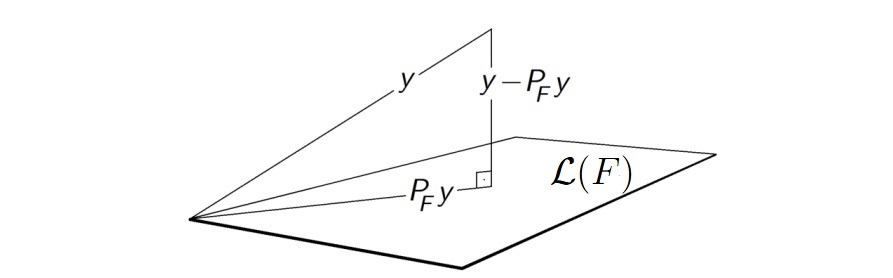
\includegraphics[scale=0.7]{MLbook/chapters/general_linear/pictures/Картинка проекции.jpg}
\end{figure}

МНК - это опускание перпендикуляра из $\mathbb{R}^l$ из $y$ на $\mathcal{L}(F)$.
 
\subsection*{Сингулярное разложение.} 

Немного математики:
Произвольная матрица $l \times n$ представима в виде \textit{сингулярного разложения}  (singular value deсomposition, SVD):
$$F = VDU^\top$$
\noindent\textbf{Основные свойства} сингулярного разложения:

$l \times n$ матрица $V = (v_1, ..., v_n)$ ортогональна, $V^\top V = I_n$, при этом столбцы $v_j$ - свобственные векторы матрицы $l \times l$-матрицы $FF^\top$.

$n \times n$ матрица $U = (u_1, ..., u_n)$ ортогональна, $U^\top U = I_n$, при этом столбцы $v_j$ - свобственные векторы $n \times n$-матрицы $F^\top F$.

$n \times n$ матрица $D$ диагональна, $diag(\sqrt{\lambda_1}, ..., \sqrt{\lambda_n})$, при этом $\lambda_j \leq 0$ - общие собственные значения $F^\top F$ и $FF^\top$.

Зачем нам это нужно? Чтобы посчитать ранее определенное решение:

$F^+ = (F^\top F)^{-1}F^\top$, применим сингулярное разложение к $F$
$$F^+ = ((VDU^\top)^\top VDU^\top)^{-1} (VDU^\top)^\top =$$ 
Воспользуемся 2 тождествами: 1)$(AB)^{-1} = B^{-1} A^{-1}, 2) (AB)^{\top} = B^{\top} A^{\top}$
По 2 применим $\top$ к внешнему и внутреннему разложениям, получим:
$$(UDV^\top VDU^\top)^{-1} UDV^\top =$$
По 1 применим возведение в $-1$ степень к большой скобке с знанием $U^{-1} = U^\top, V^{-1} = V^\top$:
$$UD^{-1}V^{-1}VD^{-1}U^{-1} UDV^\top = UD^{-1}D^{-1}DV^\top = UD^{-1}V^\top = \sum_{j = 1}^n \frac{1}{\sqrt{\lambda_j}}u_j v_j^\top$$
Тогда, тк $w^* = F^+ y$, то
$$w^* = UD^{-1}Vy = \sum_{j = 1}^n \frac{1}{\sqrt{\lambda_j}}u_j (v_j^\top y)$$
Найдем проекцию:
$$Fw^* = P_Fy = (VDU^\top) UD^{-1}Vy = VV{-1}u = \sum_{j = 1}^n v_j(v_j^\top y)$$
Найдем норму нашего решения с знанием $\|w\|^2 = w^\top W$:
$$\|w^*\|^2 = \|UD^{-1}Vy\|^2 = (UD^{-1}Vy)^\top UD^{-1}Vy =$$
$$(D^{-1}Vy)^{\top} U^\top UD^{-1}Vy = (D^{-1}Vy)^{\top} D^{-1}Vy = \|D^{-1}Vy\|^2 =  \sum_{j = 1}^n \frac{1}{\lambda_j}v_j(v_j^\top y)$$

\subsubsection*{Задача 1.} 
Имеется 2 куска сыра весами a и b. На одних и тех же весах сначала взвесили первый, потом второй, затем оба. Найдите оценку наименьших квадратов для a и b.
\noindent\textit{Решение.} Пусть показало результаты $y_1, y_2, y_3$. Положим $y = (y_1, y_2, y_3)^\top$, тогда $y = l + \varepsilon$, где $l = (a, b, a + b)^\top$. Обозначим $l = Fw$, где $w = (a, b)^\top$ и 
$$F = \begin{pmatrix}
    1 \ 0 \\
    0 \ 1 \\
    1 \ 1
\end{pmatrix}$$.

Тогда $w^* = (F^\top F) F^\top y = \begin{pmatrix}
    \frac{2}{3}y_1 - \frac{1}{3}y_2 + \frac{1}{3}y_3 \\
    -\frac{1}{3}y_1 + \frac{2}{3}y_2 + \frac{1}{3}y_3
\end{pmatrix}$

\subsubsection*{Задача 2.} Над Хлебостаном обнаружили НЛ$\Theta$ -- неопознанный летающий $\theta$чпочмак. Дрожайшее министерство, встретило НЛ$\Theta$ с хлебом солью, послав в него множество багет.
Мученые Хлебостана заметили, что $\theta$чпочмак летает на постоянной высоте, а для уклонения перемещается по какой-то странной траектории. Мученые устоноваили множество спор, на протяжении 1 прямой линии, с помощью которых зафиксировали некоторый набор позиций $\theta$чпочмака. Министерство хлебороны требует от мученых определить куда отправить багету, чтобы наконец-то сбить НЛ$\Theta$. Мученые преполагают, что НЛ$\Theta$ движется по квадрике ($ax^4 + bx^3 + cx^2 + dx + e = 0$. Помогите мученым определить расположение $\theta$чпочмака, пока их не обидели булцы.

Данные:
\begin{figure}[h]
    \centering
    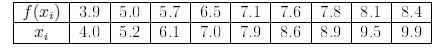
\includegraphics[scale=0.7]{MLbook/chapters/general_linear/pictures/табличка.jpg}
\end{figure}
 
\noindent\textit{Решение.} Сформулируем задачу на языке многомерной линейной регрессии. У нас есть $9$ объектов-чисел, числовые признаки которых это просто их значения на функциях $1, x, x^2, x^3, x^4$. Тогда модель может быть составлена так:
$$F = \begin{pmatrix}
    1 & 1 & \dots & 1 \\
    4.0 & 5.2 & \dots & 9.9 \\
    16.0 & 27.04 & \dots & 98.01 \\
    64.0 & 5.2^3 & \dots & 9.9^3 \\
    4.0^4 & 5.2^4 & \dots & 9.9^4
\end{pmatrix}^T, \;\; w = \begin{pmatrix}
    \beta_1 \\
    \beta_2 \\
    \beta_3 \\
    \beta_4 \\
    \beta_5
\end{pmatrix}.$$
Дальше решаем систему ища $w^*$, где $y = (f(x_1), ..., f(x_9))^\top$

\section*{Lasso-регрессия (L1-регуляризация)}

Lasso-регрессия (Least Absolute Shrinkage and Selection Operator) включает $\ell_1$-регуляризацию, которая одновременно выполняет отбор признаков и предотвращает переобучение. Задача оптимизации формулируется следующим образом:
\[
\min_{\beta \in \mathbb{R}^p} \frac{1}{2n} \sum_{i=1}^n (y_i - x_i^T \beta)^2 + \lambda \|\beta\|_1,
\]
где $\|\beta\|_1 = \sum_{j=1}^p |\beta_j|$, а $\lambda > 0$ — параметр регуляризации. Штраф $\ell_1$ приводит к занулению некоторых коэффициентов $\beta_j$, тем самым автоматически выполняя отбор признаков.

\subsection*{Задача 1}
Как на основе Lasso-регрессии определить значимость признаков в линейной модели? 

\subsection*{Задача 2}
Сохраняет ли L1-регуляризация следующие свойства оптимизационной задачи:
\begin{itemize}
    \item гладкость,
    \item выпуклость,
    \item сильную выпуклость?
\end{itemize}

\subsection*{Задача 3}
Как известно, метод SVM сводится к решению задачи квадратичного программирования. Сохраняет ли эта задача квадратичность при добавлении L1-регуляризации? Если нет, какие методы оптимизации можно использовать для эффективного решения этой задачи?

\section*{Регуляризация. Гребневая регрессия.}

Итак, мы решили задачу многомерной линейной регрессии методом наименьших квадратов. Казалось бы, что всё уже хорошо, однако в решении мы воспользовались крайне опасным инструментом -- умножением на обратную матрицу. При таком подходе можно запнуться об подводные камни. В этом разделе мы поймём суть проблемы и предложим эффективный способ с ней бороться.

\subsection*{Мультиколлинеарность и число обусловленности матрицы.}
Вспомним, как записывается решение МНК:
$$w^* = (F^T F)^{-1} F^T y, \; \|w^*\|^2 = \sum_{j=1}^n \frac{1}{\lambda_j}(v_j^T y)^2.$$
Видим проблему, если $\lambda_j$ маленькие, то решение <<взрывается>>. Это происходит, если найдется $U \in \mathbb{R}^n$ такое, что $Fu \approx 0$, то есть столбцы $F$ почти линейно зависимы. Формализуем понятие <<взрыва>> решения.

\noindent\textbf{Определение.} \textit{Числом обусловленности} 
положительно определённой квадратной матрицы $S$ называется величина
$$\mu(S) := \|S\| \cdot \|S^{-1}\|.$$

Теперь мы видим, что при умножении обратной матрицы на вектор, относительная погрешность может увеличиться в $\mu(S)$ раз:
$$\frac{\|\delta(S^{-1}u)\|}{\|S^{-1}u\|} = \frac{\|S^{-1} \delta u\|}{\|S^{-1}u\|} \leqslant \mu(S)\frac{\|\delta u\|}{\|u\|}.$$
Неравенство следует из того факта, что
$$\|S^{-1}\delta u\| \leqslant \|S^{-1}\| \cdot \|\delta u\| \;\; \text{и} \;\; \|u\| \leqslant \|S\| \cdot \|S^{-1}u\| \; \Rightarrow \; \|S^{-1}u\| \geqslant \frac{\|u\|}{\|S\|}.$$
Также здесь $\delta u$ обозначает разность между истинным значением и наблюдением.

Следовательно, положив $S := F^T F$, $u = F^T y$ и $w^* = (F^T F)^{-1} F^T y$ получим, что погрешности измерения ($\delta u$ выше) признаков $f_j(x_i)$ и ответов $y_i$ могут увеличиться в $\mu(F^T F)$ раз.

Таким образом, если матрица $F^TF$ плохо обусловлена (значение $\mu$ большое), то решение $w^*$ неустойчиво, то есть содержит большие по модулю координаты $w_j^*$. Это приводит к переобучению. Действительно, $\|Fw^* - y\|$ на обучении маленькое, а вот $\|F'w^* - y'\|$ на тесте большое, поскольку даже при небольшой вариации $F'$ по сравнению с $F$, умножение на <<большой>> вектор $w^*$ портит значения.

Чтобы побороть этот эффект применяют \textit{регуляризацию}, реализованную в \textit{гребневой регрессии}.

\subsection*{Гребневая регрессия (ridge regression).}
Метод гребневой регрессии прост, добавим штраф за увеличение $\ell_2$-нормы вектора весов $w$.
$$Q_\tau(w) = \|Fw - y\|^2 + \tau \|w\|^2 \to \min_w,$$
где $\tau$ -- неотрицательный параметр регуляризации.

Решается новая задача абсолютно также, продифференцируем по $w$:
\begin{gather*}
    \frac{\partial Q_\tau(w)}{\partial w} = 2 F^T (Fw - y) + 2\tau w = 0; \\
    w_\tau^* = (F^TF + \tau I_n)^{-1} F^Ty.
\end{gather*}
Добавку $\tau I_n$ иногда называют <<гребнем>>, оттого и <<гребневая регрессия>>.

\subsection*{Регуляризация.}
Теперь изучим подробнее, что такого нам даёт параметр регуляризации.
Давайте заметим, что мы всё ещё можем повторить предыдущее решение и применить сингулярное разложение.
\begin{gather*}
    F^TF + \tau I_n = UDV^TVDU^T + \tau I_n = UD^2U^T + \tau UI_nU^T = U(D^2 + \tau I_n)U^T; \\
    w_\tau^* = U(D^2 + \tau)^{-1}DV^Ty = \sum_{j=1}^n \frac{\sqrt{\lambda_j}}{\lambda_j + \tau}u_j(v_j^Ty); \\
    Fw_\tau^* = VDU^Tw_\tau^* = V\left[D(D^2 + \tau I_n)^{-1}D\right]V^Ty = \sum_{j=1}^n \frac{\lambda_j}{\lambda_j + \tau} v_j(v_j^Ty); \\
    \|w_\tau^*\|^2 = \|(D^2 + \tau)^{-1}DV^Ty\|^2 = y^TV\left[D(D^2 + \tau)^{-2}D\right]V^Ty = \sum_{j=1}^n \frac{\lambda_j}{(\lambda_j + \tau)^2}(v_j^Ty)^2.
\end{gather*}
Таким образом, мы устранили проблему маленьких $\lambda_j$ добавив в знаменателе $\tau$. Правда теперь $Fw^* \not= Fw_\tau^*$, зато решение стало гораздо устойчивее.

Теперь поговорим о том как выбирать параметр $\tau$. Сразу заметим, что сингулярное разложение позволяет нам не пересчитывать каждый раз $(F^TF + \tau I_n)^{-1}$, а вычислить единожды матрицы $U, D, V$, и в таком случае пересчёт $(D^2 + \tau I_n)^{-1}$ происходит за линию, так как матрицы диагональные.

Оставим часть данных под контрольную выборку, на которой будем подбирать параметр $\tau$. За счёт линейной скорости пересчёта можем реализовать эффективный поиск по сетке. Пусть $X^k = (x_i', y_i')_{i=1}^k$ -- контрольная выборка.
$$\underset{k \times n}{F'} = \begin{pmatrix}
    f_1(x_1') & \dots & f_n(x_1') \\
    \dots & \dots & \dots \\
    f_1(x_k') & \dots & f_n(x_k')
\end{pmatrix}, \quad \underset{k \times 1}{y'} = \begin{pmatrix}
    y_1' \\
    \dots \\
    y_k'
\end{pmatrix}.$$
Как долго происходит вычисление функционала $Q$ при условии, что в сетке $T$ параметров (то есть мы проверяем все $\tau$ на некотором отрезке с шагом $\frac{1}{T}$)?
$$Q(w_\tau^*, X^k) = \|F'w_\tau^* - y'\|^2 = \left\|\underset{k \times n}{\underbrace{F'U}} \underset{\text{диагональная} \; n \times n}{\underbrace{\text{diag}\left(\frac{\sqrt{\lambda_j}}{\lambda_j + \tau}\right)}}\underset{n \times 1}{\underbrace{V^Ty}} - y'\right\|^2.$$
Видим, что внутри достаточно один раз вычислить $F'U$ за $O(kn^2)$, один раз вычислить $V^Ty$ за $O(kn)$ и затем $T$ раз вычислить центральный элемент за $O(n)$ и умножить на соседей за $O(kn)$. Оставшиеся операции укладываются в $O(k)$.
$$\text{Число операций поиска по сетке:} \; O(kn^2 + knT).$$

\subsection*{Сжатие и сокращение <<эффективной размерности>>.}
Иногда эту регуляризацию называют \textit{сжатием} (shrinkage) или \textit{сокращением весов} (weight decay). Действительно, заметим, что
$$\|w_\tau^*\|^2 = \sum_{j=1}^n \frac{\lambda_j}{(\lambda_j + \tau)^2}(v_j^Ty)^2 < \sum_{j=1}^n \frac{1}{\lambda_j} (v_j^Ty)^2 = \|w^*\|^2,$$
то есть регуляризованный вектор весов строго меньше обычного.

Вместе с этим ещё говорят, что регуляризация сокращает <<эффективную размерность>>. Здесь подразумевается размерность подпространства, на которое мы проектируем с помощью оператора $F(F^TF)^{-1}F^T$. Несложное наблюдение: размерность подпространства при проекции равна следу матрицы оператора проекции.
$$\text{tr } F(F^TF)^{-1}F^T = \text{tr } (F^T F)^{-1} F^TF = \text{tr } I_n = n.$$
При использовании регуляризации:
$$\text{tr } F(F^TF + \tau I_n)^{-1}F^T = \text{tr } \text{diag}\left(\frac{\lambda_j}{\lambda_j + \tau}\right) = \sum_{j=1}^n \frac{\lambda_j}{\lambda_j + \tau} < n.$$
Выше мы пользовались свойством $\text{tr}(A_1 \dots A_m) = \text{tr}(A_m A_1 \dots A_{m-1})$.

\newpage
\subsection*{Задачи.}

\subsubsection*{Задача 1.} Как мы уже поняли, число обусловленности может быть полезной характеристикой. При этом мы говорили, что обычное решение МНК ломают маленькие собственные значение. Хочется связать эти понятия, поэтому предлагается доказать следующее утверждение для симметричной положительно определённой матрицы $S$ (это согласуется с $S := F^TF$):
$$\mu(S) = \frac{\lambda_{\max}(S)}{\lambda_{\min}(S)},$$
где $\lambda_{\max}(S)$ и $\lambda_{\min}(S)$ максимальное и минимальное собственное значение матрицы $S$ соответственно.

\noindent\textit{Решение.} Докажем сначала, что $\|S\| = \lambda_{\max}(S)$. Действительно, $S$ симметрична и положительно определена, значит существует базис, состоящий из собственных векторов матрицы $S$, обозначим их за $e_1, \dots, e_n$.
\begin{gather*}
\|S\| = \max_{u \not= 0} \frac{\|Su\|}{\|u\|} = \frac{\|\lambda_1c_1e_1 + \dots + \lambda_nc_ne_n\|}{\|c_1e_1 + \dots + c_ne_n\|} = \sqrt{\frac{\lambda_1^2c_1^2 + \dots + \lambda_n^2c_n^2}{c_1^2 + \dots + c_n^2}} \leqslant \\
\sqrt{\frac{\lambda_{\max}(S)^2(c_1^2 + \dots + c_n^2)}{c_1^2 + \dots + c_n^2}} = \lambda_{\max}(S).
\end{gather*}
Максимум достигается, если $u$ собственный вектор, соответствующий $\lambda_{\max}(S)$. Альтернативно распишем $S = C^{-1} \text{diag}(\lambda_i) C$, где $C$ -- матрица перехода к базису из собственных векторов, следовательно $S^{-1} = C^{-1} \text{diag}(1/\lambda_i) C$. Таким образом,
$$\mu(S) = \|S\| \cdot \|S^{-1}\| = \lambda_{\max}(S) \cdot \lambda_{\max}(S^{-1}) = \frac{\lambda_{\max}(S)}{\lambda_{\min}(S)}.$$
% Распишем по определению нормы матриц.
% $$\mu(S) = \|S\| \cdot \|S^{-1}\| = \max_{\|u\| = 1} \|Su\| \cdot \max_{\|u\| = 1} \|S^{-1}u\| =
% \frac{\max_{\|u\| = 1}\|Su\|}{\min_{\|v\| = 1} \|Sv\|} = \frac{\lambda_{\max}(S)}{\lambda_{\min}(S)}.$$
% Здесь мы воспользовались тем фактом, что $\displaystyle \max_{\|u\| = 1} \|S^{-1}u\| = \frac{1}{\min_{\|v\| = 1} \|Sv\|}$

\subsubsection*{Задача 2.} Заметим, что регуляризация может грубо действовать на дроби $\displaystyle\frac{\lambda_j}{\lambda_j + \tau}$, например мы точно знаем, что для дробей с достаточно большими собственными значениями в идеале надо было бы выбрать $\tau = 0$. Предложим такой способ, применим штраф покоординатно:
$$Q_\tau(w) = \|Fw - y\|^2 + \sum_{j=1}^n\tau_jw_j^2 \to \min_w.$$
Как тогда измениться решение $w_\tau^*$ и квадрат его нормы $\|w_\tau^*\|^2$?

\noindent\textit{Решение.} Это задача с подвохом. Увы, в жизни не всегда хорошо даже то, что диагонально. Казалось бы, продифференцировав всё выражение мы получим, что
$$w_\tau^* = (F^TF + \text{diag}(\tau_j))^{-1} F^Ty.$$
На этом этапе всё чисто. Однако когда мы попытаемся преобразовать это выражение через сингулярное разложение, то столкнёмся с проблемой.
$$F^TF + \text{diag}(\tau_j) = UDV^TVDU^T + \text{diag}(\tau_j) \overset{(!!!)}{=} UD^2U^T + U\text{diag}(\tau_j)U^T = \dots$$
Обратите внимание на переход с восклицательными знаками. В теории выше мы воспользовались переходом $U I_n U^T = I_n$ и для единичной матрицы он верен, но вот для произвольной диагональной, увы, уже нет.
$$\begin{pmatrix}
    \frac{1}{2} & -\frac{\sqrt{3}}{2} \\
    \frac{\sqrt{3}}{2} & \frac{1}{2}
\end{pmatrix} \cdot \begin{pmatrix}
    1 & 0 \\
    0 & 2
\end{pmatrix} \cdot \begin{pmatrix}
    \frac{1}{2} & \frac{\sqrt{3}}{2} \\
    -\frac{\sqrt{3}}{2} & \frac{1}{2}
\end{pmatrix} = \begin{pmatrix}
    \frac{7}{4} & -\frac{\sqrt{3}}{4} \\
    -\frac{\sqrt{3}}{4} & \frac{5}{4}
\end{pmatrix}.$$

\subsubsection*{Задача 3.} В древних скрижалях Самсууса, первого пекаря Хлебостана, скрыта тайна идеальной самсы. Команда археологов университета Зерноэматики смогла перевести почти весь рецепт, но вот беда, коэффициенты в одном из уравнений для выпечки стёрлись без шанса на восстановление. Сейчас его можно записать как $f(x) = \beta_1 + \beta_2 x + \beta_3 x^2 + \beta_4 \cos x$. К счастью команда нашла способ промоделировать поведение левой части (то есть $f(x)$) с некоторой точностью для всех значений $x \in [0, 1]$ с шагом $0.1$. Ваша задача построить модель, которая сможет предсказать остальные значения этой функции $f(x)$. Ответьте на вопрос, стоит ли применять регуляризацию. А если бы значения $f(x)$ приходили из другого множества?

\noindent\textit{Решение.} Сформулируем задачу на языке многомерной линейной регрессии. У нас есть $11$ объектов-чисел, числовые признаки которых это просто их значения на функциях $1, x, x^2, \cos x$. Тогда модель может быть составлена так:
$$F = \begin{pmatrix}
    1 & 1 & \dots & 1 \\
    0 & 0.1 & \dots & 1 \\
    0 & 0.01 & \dots & 1 \\
    \cos 0 & \cos 0.1 & \dots & \cos 1
\end{pmatrix}^T, \;\; w = \begin{pmatrix}
    \beta_1 \\
    \beta_2 \\
    \beta_3 \\
    \beta_4
\end{pmatrix}.$$
Главный вопрос, стоит ли применять регуляризацию? Конечно, вспомним, что $\cos x = 1 - \frac{x^2}{2} + o(x^3)$ в окрестности точки $0$, а значит у нас имеется почти линейная зависимость $1, 3$ и $4$ столбца (обратите внимание, что матрица транспонирована). Ну и теперь мы видим, когда регуляризация действительно нужна, а именно, когда значения $x$ достаточно малы (для $|x| < 1$ формула Тейлора аппроксимирует очень хорошо). Поскольку $|\cos(x)| \leqslant 1$, то уже для значений $|x| > 2$ разложение в ряд Тейлора выше ведёт себя плохо, и можно не применять регуляризацию. В любом случае, вы всегда сможете понять, что зависимость имелась, если значения $w^*$ окажутся очень большими.
